\documentclass[turkish]{report}

\usepackage{babel}
\usepackage[utf8]{inputenc}
% Title Page
\title{Modal Analiz 2. Ödevi}
\author{Burak ER}
\usepackage{hyphenat}

\usepackage{psfrag}

\usepackage{amsmath}

\usepackage{amssymb}

\usepackage{pstricks, pst-node, pst-plot, pst-circ}

\usepackage{moredefs}

\usepackage[bookmarks=true,bookmarksopenlevel=3,bookmarksopen=true,        bookmarksnumbered=true,linkbordercolor={0 1 0},citebordercolor={0 1 0},urlbordercolor={0 0 0},pdfstartview={FitH},linktocpage=true,plainpages=false]{hyperref}

\usepackage{cleveref}

\usepackage{graphicx}

\usepackage{epstopdf}

\usepackage{epsfig}

\usepackage{algorithm}


\usepackage{program}

\usepackage{graphicx}

\usepackage{caption}


\usepackage{caption}
\usepackage{subcaption}

\usepackage[autolinebreaks,useliterate]{mcode}

\crefname{lstlisting}{listing}{listings}

\Crefname{lstlisting}{Listing}{Listings}

\begin{document}


\maketitle
\section*{Problem 1}
Sızıntı(spectral  leakage)kavramını teorik temelleri ile birlikte  açıklayınız. Sızıntıyı azaltmak için neler yapılır? Pencereleme  (windowing) işlemini açıklayınız ve farklı pencerelerin özelliklerini, kullanım alanlarını, avantaj ve dezavantajlarını izah ediniz. 
\begin{center}
\subsection*{Sonuçlar 2}
\end{center}
Dijital olarak ölçülen bir sinyal sonlu sayıda ölçüldüğünden dolayı, bir takım problemler ortaya çıkmaktadır.
Bu problemlerden birisi de sızıntıdır. Sızıntı sonlu sayıdaki ölçümden kaynaklanan belli bir frekanstaki sinyal gücünün komşu-
luğundaki diğer frekanslara da taşması olayıdır. Sızıntının sebebi geçici bir sinyalin belli bir aralıkta kesilmesi ve bu aralıkta sinyalin periyodik olduğu kabulüdür.\\

Gerçek zamanda örnek bir sinyal ve onun belli bir aralıkta kesilmiş hali şekil-\ref{fig:leakage}'de gösterilmiştir. Kesilmiş sinyalin frekans bileşeni dalgalı bir hal almaktadır.
Zaman domeninde sinyalin kesilmesi işlemine pencereleme denmektedir.
\begin{figure}[ht!]
\centering
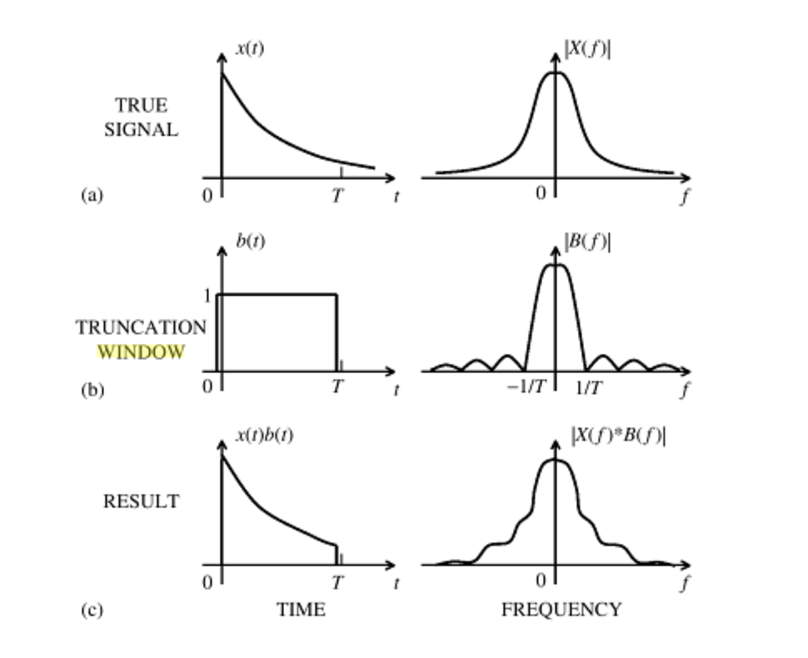
\includegraphics{./Figures/leakeage.eps}
\caption{Bir sinyal ve sızıntıya neden olan kesilmiş gösterimi\cite{norton2003fundamentals}}
\label{fig:leakage}
\end{figure}

Sürekli bir sinyalin kesikli temsili de pencereleme işlemi yapılmış bir sinyal olacağından, zaman domenindeki tüm sinyallerin digital gösterimi sızıntı içerir. Sızıntının giderilmesi için pencereleme fonksiyonları kullanılmaktadır. Bu fonksiyonlar zamana bağlı bir fonksiyona, spektral domendeki bir fonksiyona veya bir korelasyon fonksiyonuna uygulanmaktadır\cite{norton2003fundamentals}. Kullanılan tüm pencere fonksiyonları üçgen tabanlıdırlar. Bazı pencereleme fonksiyonları aşağıda verilmiştir\cite{wiki:002}.


\begin{itemize}
\item[]{Polinom tabanlı pencereler:}
\begin{itemize}
\item{ Dikdörtgen}
\item{ Üçgen}
\item{ Parzen }
\item{ Welch}
\item{ Genelleştirilmiş Hamming }
\item{ Hann (Hanning)}
\item{ Hamming}
\end{itemize}

\item[]{Higher-order generalized cosine windows:}
\begin{itemize}
\item Blackman 
\item Nuttall 
\item Blackman–Nuttall 
\item Blackman–Harris 
\item Flat top 
\item Rife–Vincent 
\end{itemize}
\end{itemize}

\section*{Problem 2}
Otokorelasyon ve çapraz korelasyon fonksiyonlarını, otospektrum ve çapraz spectrum fonksiyonlarını ve bunların özelliklerini matematiksel açıklamalarla anlatınız.  Modal  analizde  kullanılan  FRF versiyonlarından $\mathrm{H_1}$ ve $\mathrm{H_2}$'yi açıklayınız.
\begin{center}
\subsection*{Sonuçlar}
\end{center}
~\\
Korelasyon, olasılık kuramı ve istatistikte iki rassal değişken arasındaki doğrusal ilişkinin yönünü ve gücünü belirtir. Genel istatistiksel kullanımda korelasyon, bağımsızlık durumundan ne kadar uzaklaşıldığını gösterir\cite{wikikorelasyon}. 
\\

Korelasyon, benzer şekilde sinyal işlemede de iki sinyalin arasındaki doğrusal ilişkiyi ve gücü göstermektedir. Sinyal işlemede korelasyon iki sinyal arasında benzerlik olup olmadığının bilinmesi için kullanılmaktadır\cite{realtimesignalprocessing}. Dolayısıyla korelasyon ile bir sinyalin diğer bir sinyalin içeriğinde mevcut olup olmadığının tespiti yapılmaktadır. Sinyal işlemede iki çeşit korelasyon fonksiyonu mevcuttur. Bunlar: 
\\

\begin{itemize}
\item çapraz korelasyon
\item otokorelasyon 
\end{itemize}

fonksiyonlarıdır. 

\subsubsection*{Çapraz Korelasyon}

Çapraz korelasyon fonksiyonu bir sinyalin başka bir sinyal ile, bu sinyale zaman gecikmesi eklenerek, eklenen gecikmeye bağlı benzerliklerini temsil eder. Herhangi bir  $f\left(t\right)$ ve $g\left(t\right)$ fonksiyonu için, çapraz korelasyon fonksiyonu

\begin{align}
(f \star g)(\tau)\ \stackrel{\mathrm{tanım}}{=} \int_{-\infty}^{\infty} f^*(t)\ g(t+\tau)\,dt,
\label{esitlik:caprazkorelasyon}
\end{align}
\\
olarak ifade edilmektedir. Burada $f^*$, $f$ fonksiyonun complex eşleniği, $\tau$ ise zaman gecikmesidir. Eşitlik \ref{esitlik:caprazkorelasyon}' den de görüldüğü üzere herhangi iki fonksiyonun correlasyonu zamanda öteleme değeri $\tau$' ya bağlıdır.

Çapraz korelasyon fonksiyonu önemli özellikleri:\\

\begin{itemize}
\item[]{Çapraz korelasyon ile konvolusyon ilişkisi}
\begin{itemize}
\item[]{$f\star g = f^*(-t)*g$}
\end{itemize}
\item[]{Çapraz korelasyonun frekans domenindeki eşiti}
\begin{itemize}
\item[]{$\mathcal{F}\{f\star g\}=(\mathcal{F}\{f^*\}) \cdot \mathcal{F}\{g\}$}
\end{itemize}
\item[]{Çapraz korelasyonun değişme özelliği olmaması}
\begin{itemize}
\item[]{$f\star g \neq g\star f$}
\end{itemize}
\end{itemize}

\subsubsection*{Otokorelasyon}

Otokorelasyon fonksiyonu bir fonksiyonun kendisiyle çapraz korelasyonunu ifade eden fonksiyondur ve 

\begin{align}
(f \star f)(\tau)\ \stackrel{\mathrm{tanım}}{=} \int_{-\infty}^{\infty} f^*(t)\ f(t+\tau)\,dt,
\label{esitlik:otokorelasyon}
\end{align}
\\
eşitliğinden elde edilir. Otokorelasyon fonksiyonu bir sinyalin zamanda ötelenmiş haliyle korelasyonunu belirtmektedir. Sinyal içerisindeki tekrarların tayini ve yerinin tespiti için önemlidir. Ayrıca sinyalin komşuluklarındaki kendi değerleri ile benzeşimini de belirtmektedir. Bu benzeşime göre sinyalin rastgele olup olmadığı kestirilebilmektedir. Hızlı değişen sinyalin otokorelasyonu az olurken, yavaş değişen sinyalin otokorelasyonu fazla olmaktadır. En fazla otokorelasyon sıfır zaman ötelenmesinde gerçekleşmektedir. Otokorelasyon fonksiyonun davranışı için örnek sinyaller şekil \ref{fig:autocorrelation}'de verilmiştir.

\begin{figure}
\centering
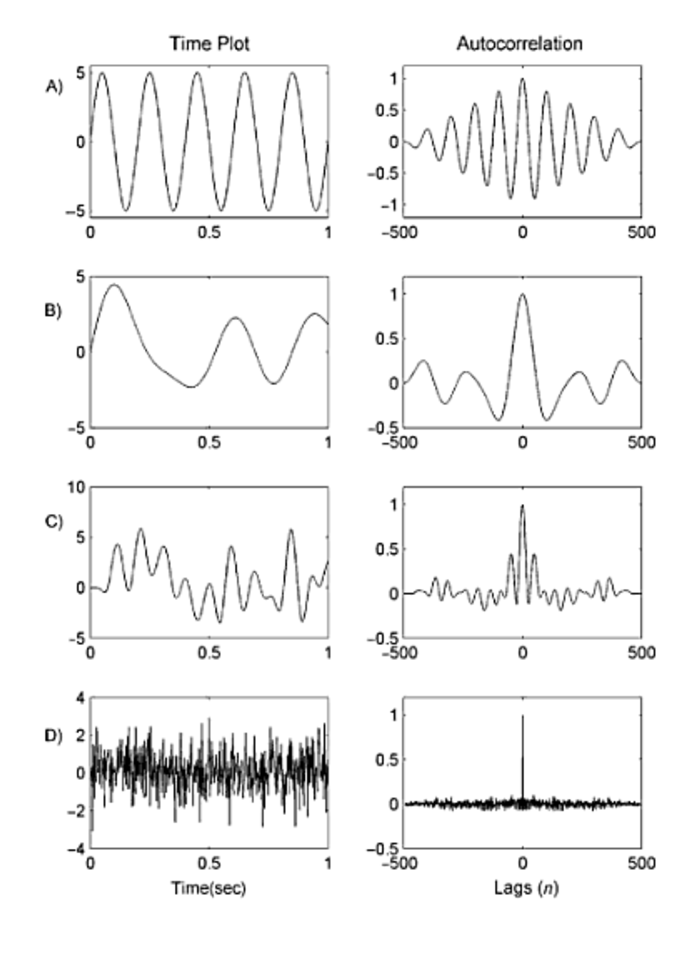
\includegraphics{./Figures/autocorrelation.eps}
\caption{Bazı fonksiyonlar ve otokorelasyonları \cite{semmlow2012signals}}
\label{fig:autocorrelation}
\end{figure}

\subsubsection*{Çaprazspektrum ve Otospektrum}
Çaprazspektrum, herhangi iki fonksiyonun çapraz korelasyonlarının Fourier dönü-şümüdür ve frekans domeninde iki fonksiyonun Fourier dönüşümlerinin çarpımı şeklindedir. Çaprazspektrum 
\begin{eqnarray}
\begin{split}
\mathrm{S_{fg}}\left(\omega\right)&=\mathcal{F}\left[\;f\;\star\; g\;\right]\\&=\mathcal{F}\left[\;f^*\;\right] \mathcal{F}\left[\;g\;\right]
\end{split}
\end{eqnarray}
eşitliğinden bulunur. Çaprazspektrum, çapraz korelasyon fonksiyonun frekans domenindeki ifadesidir. Aynı şekilde, otospektrum da bir fonksiyonun otokorelasyonun Fourier dönüşümüdür ve
\begin{eqnarray}
\begin{split}
\mathrm{S_{ff}}\left(\omega\right)&=\mathcal{F}\left[\;f\;\star\; f\;\right]\\&=\mathcal{F}\left[\;f^*\;\right] \mathcal{F}\left[\;f\;\right]
\end{split}
\end{eqnarray}
eşitliği kullanılarak bulunur. \\

Çapraz spektrum ve otospektrum kullanılarak oluşturulan ve modal analizde kullanılan frekansa bağlı $\mathrm{H_1}$ ve $\mathrm{\mathrm{H_2}}$ fonksiyonları, ele alınan sistemin çıkış/giriş oranını temsil etmektedir. İfadeleri $x\left(t\right)$ ve $f\left(t\right)$ çıkış ve giriş fonksiyonları olmak üzere
\begin{eqnarray}
\begin{split}
\mathrm{H_1}\left(\omega \right)&=\frac{\mathrm{S_{XF}}}{\mathrm{S_{FF}}}\\
\mathrm{H_2}\left(\omega \right)&=\frac{\mathrm{S_{XX}}}{\mathrm{S_{XF}}}
\end{split}
\end{eqnarray}
eşitlikleri ile verilmektedir. Burada, giriş ve çıkış fonksiyonlarında herhangi bir gürültü olmaması durumunda $\mathrm{H_1}$ ve $\mathrm{H_2}$ sistemin frekans cevabı fonksiyonuna eşit olacaktır. Ancak gürültü varsa $m\left(t\right)$ ve $n\left(t\right)$ sırasıyla giriş ve çıkıştaki parazit fonksiyonları olmak üzere
\begin{eqnarray}
\begin{split}
\mathrm{H_1}\left(\omega \right) &= H\left(\omega \right)\left[1+\frac{\mathrm{S_{MM}}}{\mathrm{S_{FF}}}\right]^{-1}\\
\mathrm{H_2}\left(\omega \right) &= H\left(\omega\right)\left[1+\frac{\mathrm{S_{NN}}}{\mathrm{S_{XX}}}\right]
\end{split}
\label{equ:h1veh2parazitli}
\end{eqnarray}
eşitliklerine sahip olmaktadırlar. Denklem \ref{equ:h1veh2parazitli}' den görüldüğü üzere $\mathrm{H_1}$ ve $\mathrm{H_2}$ parazitlerin ve giriş ve çıkış fonksiyonlarının otospektrumlarına bağlı olmaktadır. $\mathrm{H_1}$ giriş parazit fonksiyonu otospektrumu ile giriş fonksiyonu otospektrumu oranına bağlı olarak gerçek frekans cevap fonksiyonundan saparken, $\mathrm{H_2}$ çıkış parazit fonksiyonu ve çıkış fonksiyonu otospektrumu oranına bağlı olarak sapmaktadır. Bu özellik parazit/gerçek sinyal oranının küçük olduğu data kullanılarak frekans cevabı fonksiyonun iyi bir şekilde bulunmasını mümkün kılmaktadır. Uygulamada rezonans noktalarında $\mathrm{H_2}$ kullanılırken, antirezonans civarında $\mathrm{H_1}$ in kullanılması uygundur.
\bibliographystyle{plain}
\bibliography{biblio}

\end{document}          


